\documentclass[a4paper,12pt]{article}
\usepackage{graphicx}
\usepackage[left=2cm,top=2cm,bottom=2.2cm,right=2cm]{geometry}
\usepackage[utf8]{inputenc}
\usepackage[T1]{fontenc}
\usepackage{lmodern}
\usepackage[portuguese,brazil]{babel}

\usepackage{amsmath}
\usepackage{slashbox}
\usepackage{array}
\usepackage{icomma} % para vírgula decimal / decimal comma
\usepackage{enumerate}

\newcounter{questao}
\setcounter{questao}{0}
\newcommand{\questao}{%
\vspace{12pt}%
\refstepcounter{questao}%
\noindent%
\textbf{Questão \arabic{questao}.}%
{ }%
}

\begin{document}
\begin{center}
\Large{Circuitos Digitais -- Exercícios da Aula 15}
\end{center}

\questao Para cada mapa de Karnaugh abaixo, obtenha a expressão mais simples na forma de soma de produtos.

\includegraphics[scale=0.9]{images/karnaugh}

\newpage

\questao Construa o mapa de Karnaugh para cada função abaixo e
obtenha a expressão mais simples na forma de soma de produtos. Os
estados que não estão representados devem ser considerados como
``don't care'' no mapa de Karnaugh.\\

\hfill
(a) \begin{tabular}{ccc||c}
X & Y & Z & W \\
\hline
0 & 0 & 0 & 0 \\
0 & 0 & 1 & 0 \\
0 & 1 & 0 & 1 \\
0 & 1 & 1 & 0 \\
1 & 0 & 0 & 1 \\
1 & 1 & 0 & 1 \\
\end{tabular}
\hfill
(b) \begin{tabular}{ccc||c}
A & B & C & X \\
\hline
0 & 0 & 1 & 0 \\
0 & 1 & 1 & 0 \\
1 & 0 & 0 & 1 \\
1 & 0 & 1 & 0 \\
1 & 1 & 0 & 1 \\
1 & 1 & 1 & 0 \\
\end{tabular}
\hfill
(c) \begin{tabular}{ccc||c}
X & $Q_1$ & $Q_0$ & $Y$ \\
\hline
0 & 0 & 1 & 0 \\
0 & 1 & 0 & 1 \\
0 & 1 & 1 & 0 \\
1 & 0 & 0 & 1 \\
1 & 1 & 0 & 1 \\
\end{tabular}
\hspace*{\fill}\\[12pt]

\hspace*{\fill}
(d) \begin{tabular}{ccc||cc}
X & $Q_1$ & $Q_0$ & $Y_1$ & $Y_0$ \\
\hline
0 & 0 & 0 & 1 & 0 \\
1 & 0 & 0 & 0 & 1 \\
1 & 1 & 1 & 0 & 0 \\
1 & 1 & 0 & 1 & 1 \\
\end{tabular}
\hfill
(e) \begin{tabular}{cccc||c}
A & B & C & D & X \\
\hline
0 & 0 & 0 & 0 & 0 \\
0 & 0 & 0 & 1 & 0 \\
0 & 0 & 1 & 0 & 0 \\
0 & 1 & 0 & 0 & 0 \\
0 & 1 & 0 & 1 & 0 \\
0 & 1 & 1 & 0 & 0 \\
1 & 0 & 0 & 0 & 0 \\
1 & 0 & 0 & 1 & 0 \\
1 & 0 & 1 & 0 & 0 \\
1 & 1 & 1 & 0 & 1 \\
\end{tabular}
\hfill
(f) \begin{tabular}{cccc||cc}
$X_2$ & $X_1$ & $Q_1$ & $Q_0$ & $Y_2$ & $Y_1$ \\
\hline
0 & 0 & 0 & 1 & 0 & 1 \\
0 & 0 & 1 & 1 & 0 & 1 \\
0 & 1 & 0 & 0 & 0 & 0 \\
0 & 1 & 0 & 1 & 0 & 0 \\
0 & 1 & 1 & 0 & 0 & 0 \\
1 & 0 & 0 & 0 & 1 & 1 \\
1 & 0 & 0 & 1 & 0 & 0 \\
1 & 0 & 1 & 0 & 1 & 0 \\
1 & 0 & 1 & 1 & 0 & 0 \\
1 & 1 & 0 & 0 & 0 & 1 \\
1 & 1 & 0 & 1 & 0 & 0 \\
1 & 1 & 1 & 0 & 0 & 0 \\
1 & 1 & 1 & 1 & 0 & 1 \\
\end{tabular}
\hspace*{\fill}

\noindent\hrulefill

\noindent
\begin{minipage}{0.47\textwidth}
\questao Projete uma máquina de estado cuja transição entre os
estados é dada pelo diagrama ao lado. Ela deverá possuir duas entradas,
$Ck$ (clock) e $X$, e uma saída $Z$. Use flip-flops D.
\end{minipage}
\hfill
\begin{minipage}{0.45\textwidth}
% Fonte: http://www.allaboutcircuits.com/vol_4/chpt_11/5.html
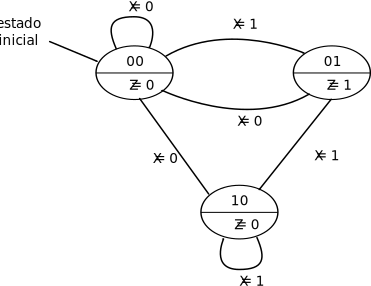
\includegraphics[width=\textwidth]{images/questao3}
\end{minipage}

\noindent\hrulefill

\questao Usando flip-flops D, projete uma máquina de estado com $2$
entradas, $Ck$ (clock) e $d$ (um bit de dado) e $n$ saídas
$Q_{n-1}, Q_{n_2}, \ldots, Q_1, Q_0$. A cada
borda de descida do clock, as saídas devem mudar de acordo com a
seguinte tabela de transição:\\

\hspace*{\fill}
\begin{tabular}{cccccc||cccccc}
\multicolumn{6}{c||}{estado atual} & \multicolumn{6}{c}{próx. estado} \\
$Q_{n-1}$ & $Q_{n-2}$ & \ldots & $Q_2$ & $Q_1$ & $Q_0$ &
	$Y_{n-1}$ & $Y_{n-2}$ & \ldots & $Y_2$ & $Y_1$ & $Y_0$ \\
\hline
$a_{n-1}$ & $a_{n-2}$ & \ldots & $a_2$ & $a_1$ & $a_0$ &
	$d$       & $a_{n-1}$ & \ldots & $a_3$ & $a_2$ & $a_1$
\end{tabular}
\hspace*{\fill}\\[12pt]

Ou seja, a cada borda de descida do clock, os bits das saídas
são deslocados uma posição para a direita. Os bits $a_{n-1}$ $a_{n-2}$
\ldots $a_1$ $a_0$ são um numeral binário armazenado previamente
nos flip-flops D.

\end{document}

